\documentclass{article}
\usepackage{fancyvrb}
\usepackage{a4wide}
\usepackage[T1]{fontenc}
\usepackage[utf8]{inputenc}
\usepackage[french]{babel}
\usepackage{empheq}
\usepackage{mathtools, bm}
\usepackage{amssymb, bm}
\usepackage{graphicx}
\usepackage{caption}
\usepackage{subcaption}
\usepackage{hyperref}
\usepackage{csvsimple}
\usepackage{float}

\title{\textbf{\Huge  Université Paris Saclay}\\ Rapport IAS}
\author{Guillaume Abadie, Jérôme Coquisart, Mathis Dupont, Martin Vitani}
\date{Année 2021}


\begin{document}
    \maketitle
    \tableofcontents

    \section{Introduction au problème}
    La ville de Chicago a un ratio de crimes, surtout sur les crimes violents, au dessus de la moyenne
    nationale des États-Unis.
    Les crimes dans la ville ont été collectés dès le début du 20ème siècle pour essayer de 
    comprendre pourquoi la ville était sujette à autant de violence.
    Le dataset correspond aux crimes commis entre 2001 et 2020, et contient environ 
    7 millions d'entrées.
    Tous les jours, la police de Chicago alimente la base de donnée avec les nouveaux crimes commis
    dans la ville. Seuls les meurtres ne sont pas comptabilisé dans la base de donnée.

    \section{Aperçu du dataset}
    \begin{figure}[H]
            \centering
	    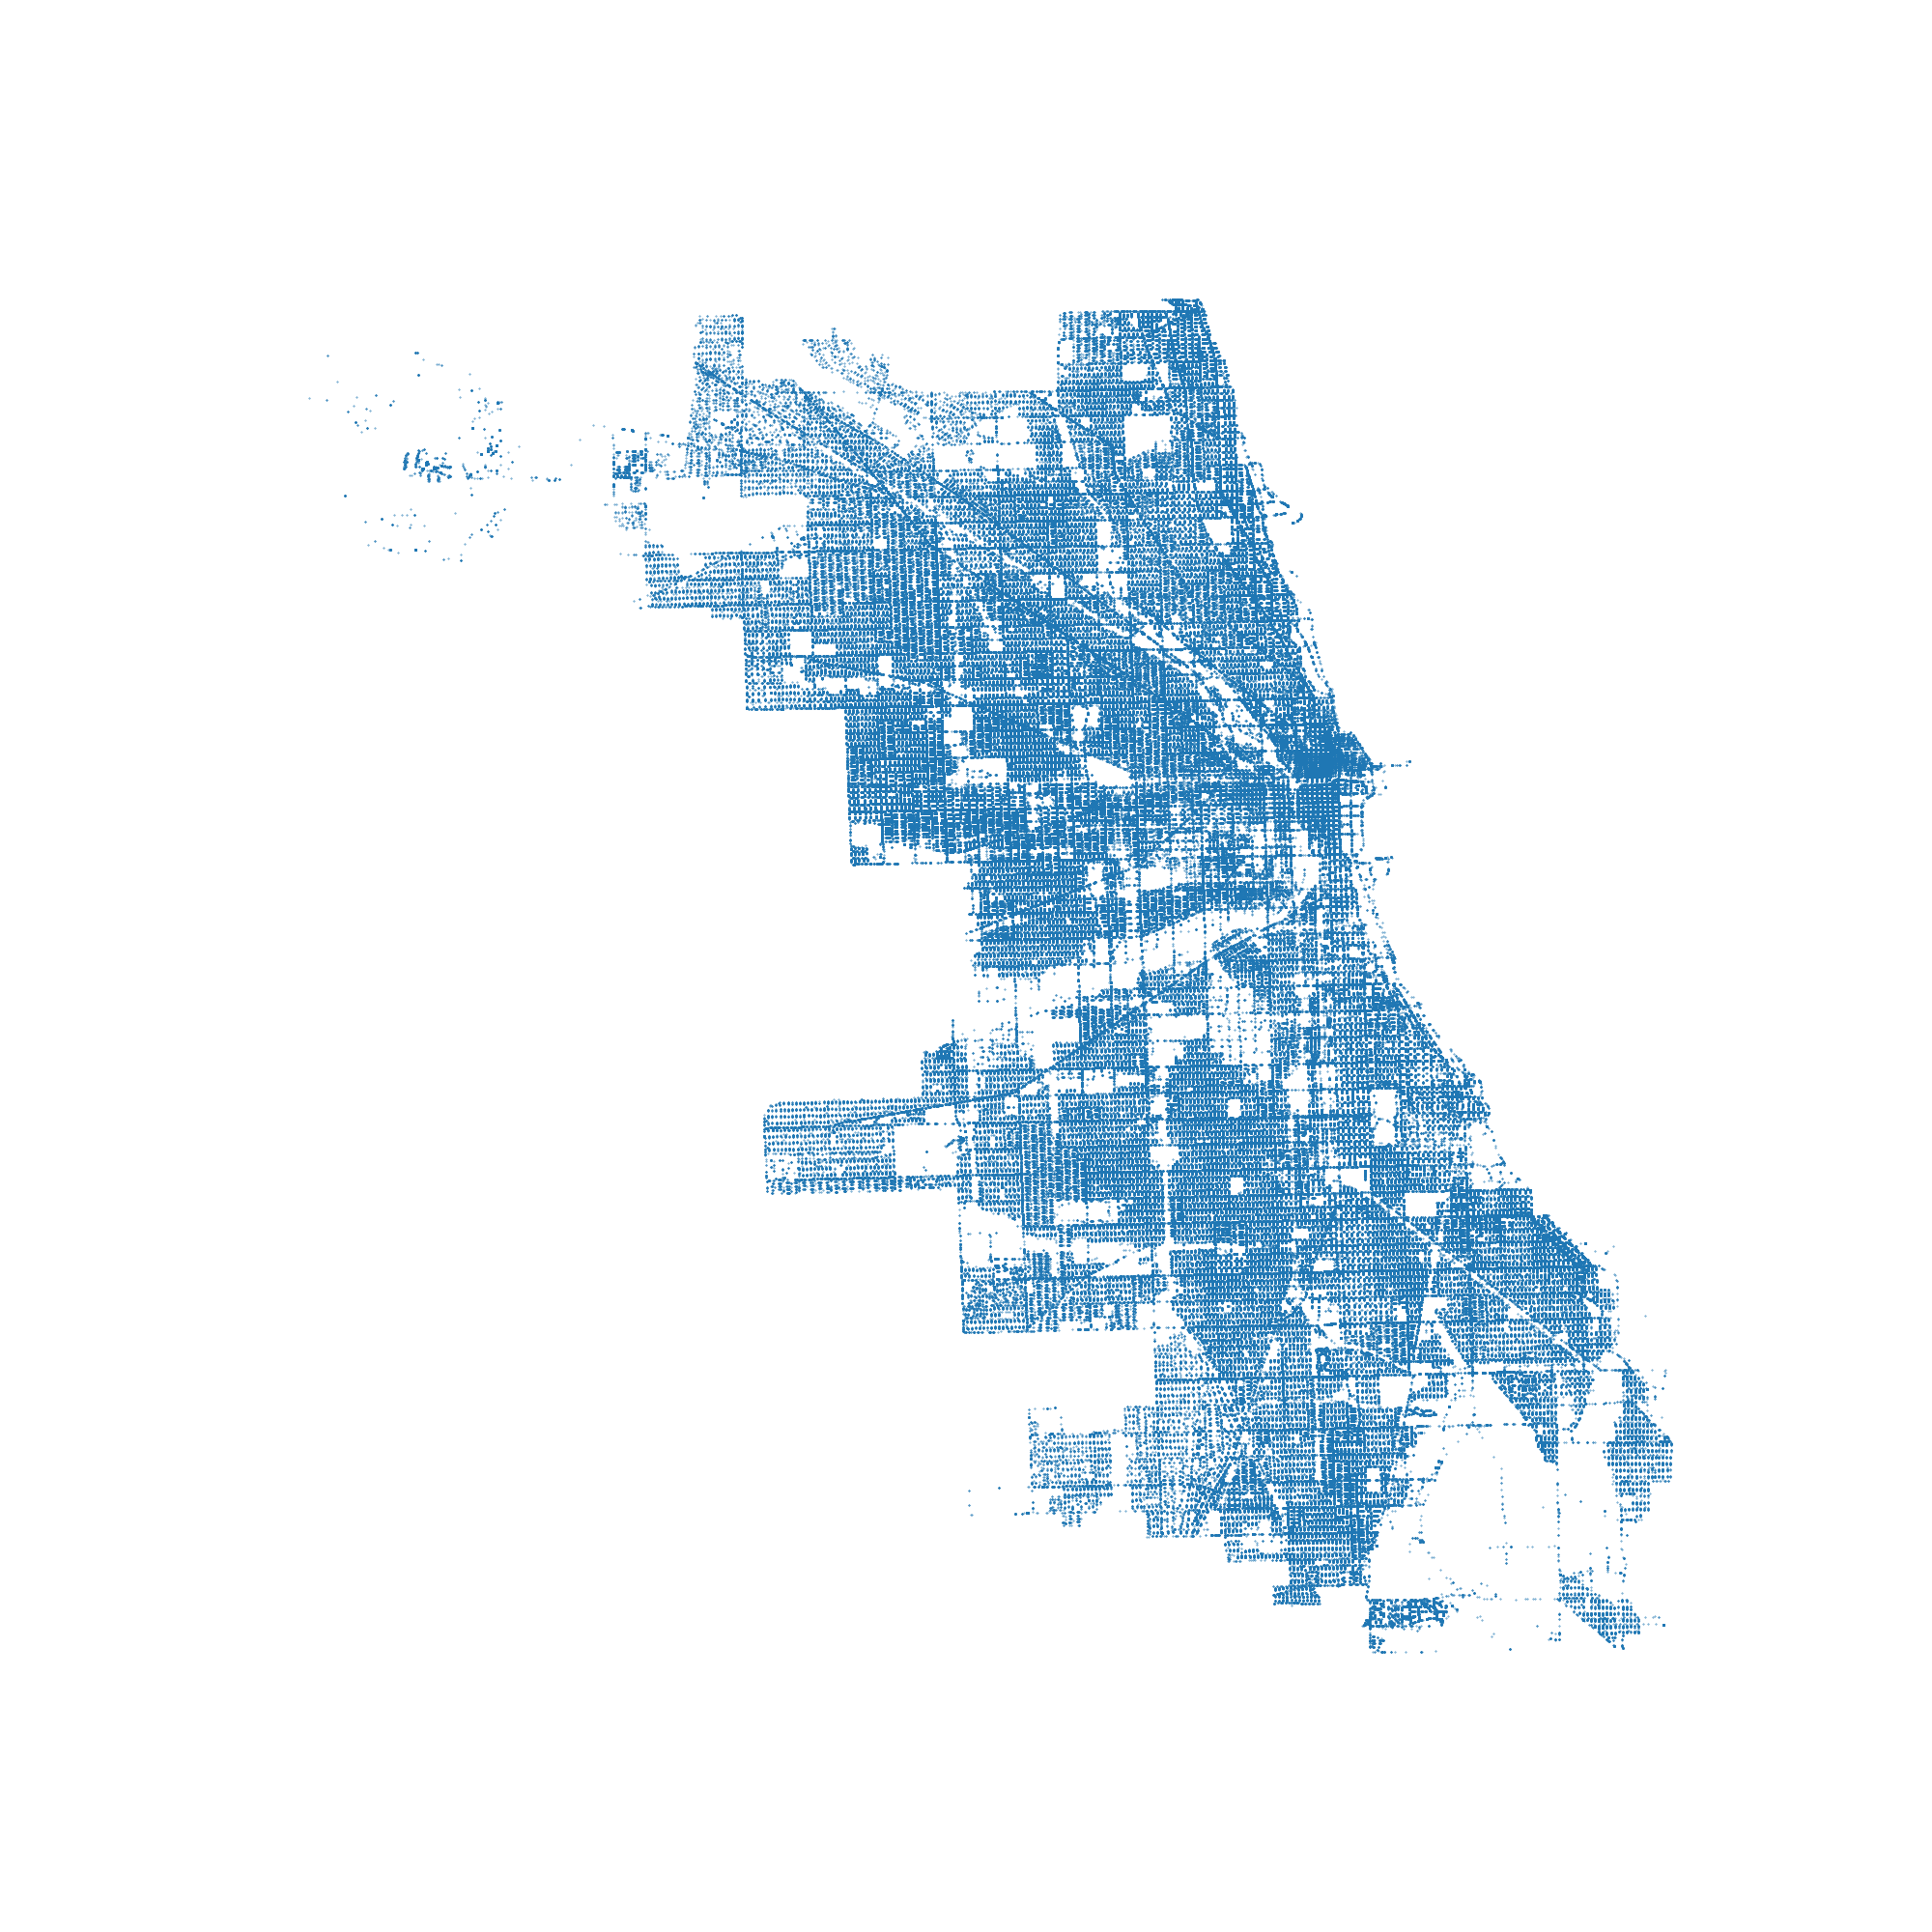
\includegraphics[scale=.2]{carte_chicago.png}
	    \caption{Carte représentant l'ensemble des crimes commis à Chicago}
    \end{figure}
    Sur cette carte, chaque point représente un crime.

    \section{Définition du problème}
    Notre problème sera le suivant. Il s'agira de déterminer si il y aura
    oui ou non une arrestation à la suite d'un crime. 
    Pour être plus précis, étant donné le lieu, la description et la date du crime, 
    il faudra dire si cela va mener à l'arrestation d'un suspect.
    C'est une tâche de classification
    binaire, en apprentissage supervisé.

    \section{Préprocessing}
    Comme le dataset contenait peu de features, 
    nous avons effectué plusieurs modifications sur le dataset avec d'entrainer notre modèle.
    De plus, certaines features étaient uniques pour chacun de nos crimes.

    Nous avons tout d'abord supprimer les données qui contenaient des features vides, et nous avons
    équilibré le dataset.
    Cela a été fait avec des commandes shell pour la rapidité et la simplicité. On rappelle que notre dataset contient 7 millions d'entrées à la base.
    Voici les commandes effectuées.

    \begin{Verbatim}
	## Nettoyer les données
	grep -v -E '(,0,0,2)|(,,)' Crimes2001.csv  > CrimesClean.csv
	
	## Equilibrer les données
	# Ici on sépares à l'aide d'expressions régulières les arrested et les non arrested
	grep -E '^(([^,]*,)|("[^"]*",)){8}false' Crimes100K.csv > CrimesCleanNonArrested.csv
	grep -E '^(([^,]*,)|("[^"]*",)){8}true' Crimes100K.csv > CrimesCleanArrested.csv
	
	# Ici on recombine en n'oubliant pas le header contenant le nom des features
    	head -n 1 CrimesClean.csv > CrimesEq.csv
	n=$(wc -l CrimesCleanArrested.csv | grep -E -o '[0-9]+ ')
	cp CrimesCleanArrested.csv tmp.csv
	shuf -n $n CrimesCleanNonArrested.csv >> tmp.csv
	shuf tmp.csv >> CrimesEq.csv
\end{Verbatim}

    Ensuite, en python, nous avons supprimé les features uniques et celles qui se répétaient
    \begin{itemize}
	    \item ID
	    \item Case Number
	    \item Block
	    \item Updated On
	    \item Longitude
	    \item Latitude
	    \item Location
    \end{itemize}
    À partir de la feature date, nous avons extrait les features suivantes
    \begin{itemize}
	    \item Part of the day
	    \item Weekday
	    \item Weekend
	    \item Month
	    \item Hour
    \end{itemize}
    Enfin, à partir des coordonnées géographiques, nous avons appliqué un algorithme de k-moyennes pour séparer les zones de Chicago et en déduire une nouvelle feature Cluster. 
    Voici ce que l'on obtiens lorsque l'on affiche la localisation des crimes en fonction de leurs clusters.
    \begin{figure}[H]
            \centering
	    \includegraphics[scale=.2]{carte_densité.png}
	    \caption{Clusters des crimes de Chicago}
    \end{figure}

    \section{Choix d'algorithme}
    Pour classifier nos crimes, nous utilisons le DecisionTree et le modèle Gaussien Naïf.
    Différentes fonctions dans le fichier main.py nous ont permis de déterminer les meilleurs
    hyper-paramètres à choisir pour le DecisionTree.
    \begin{figure}[H]
            \centering
	    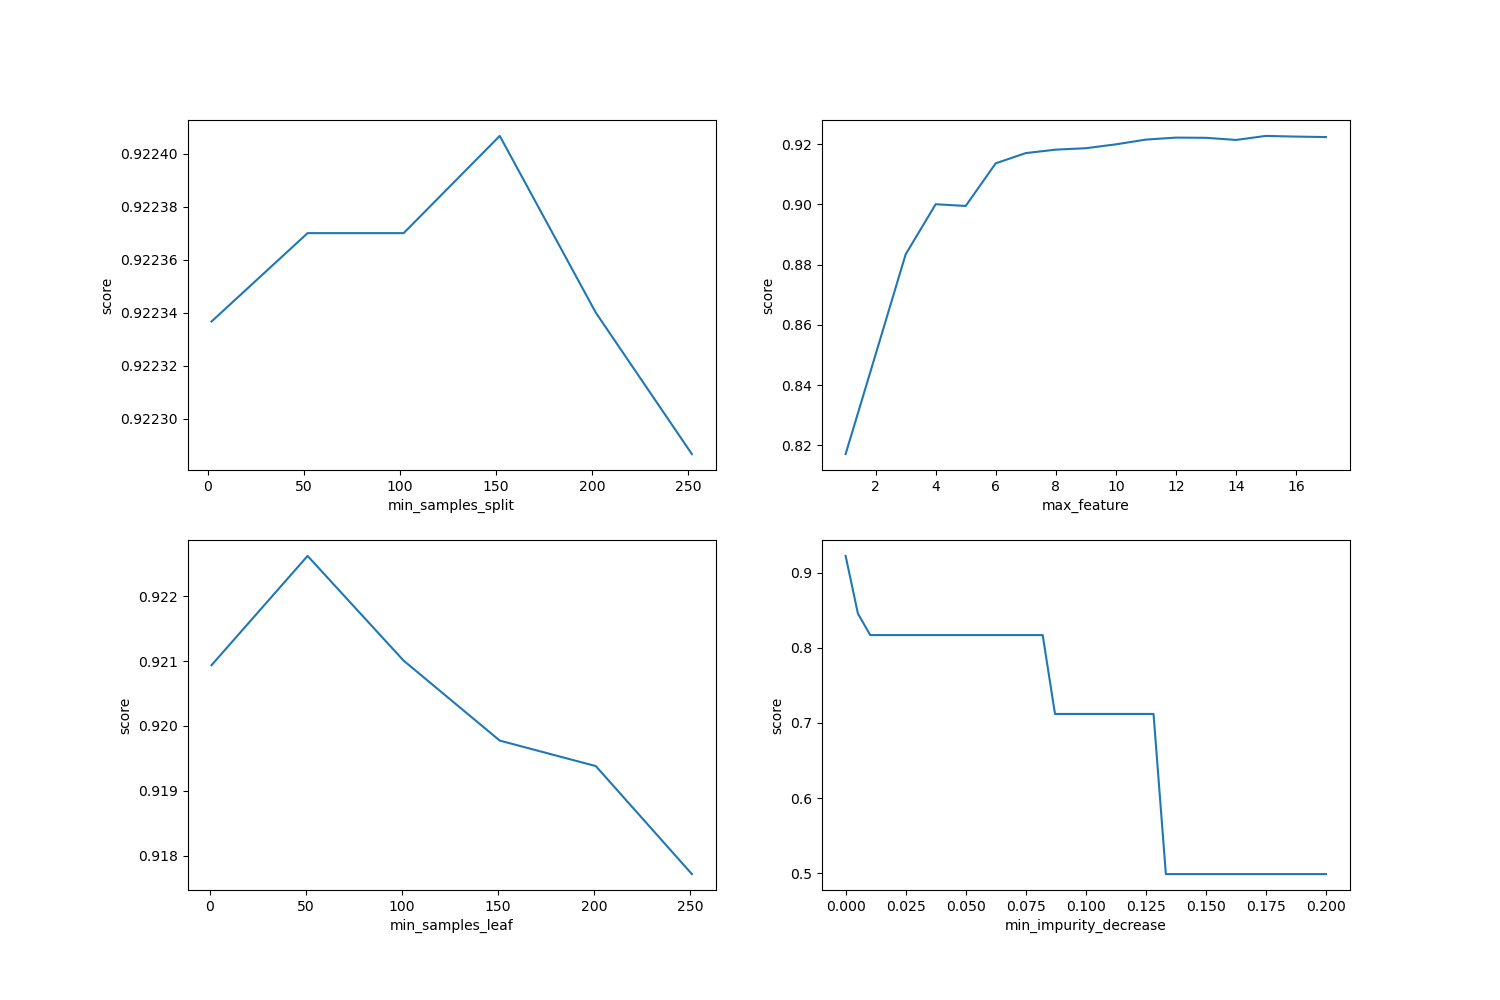
\includegraphics[scale=.4]{bestParamDecisionTree.png}
	    \caption{Cross-validation pour le DecisionTree}
    \end{figure}

    \section{Comparaison des modèles}

    \section{Présentation des résultats}

    \section{Conclusion}

\end{document}
